\documentclass[
  bibliography=totoc,     % Literatur im Inhaltsverzeichnis
  captions=tableheading,  % Tabellenüberschriften
  titlepage=firstiscover, % Titelseite ist Deckblatt
]{scrartcl}

% Paket float verbessern
\usepackage{scrhack}

% Warnung, falls nochmal kompiliert werden muss
\usepackage[aux]{rerunfilecheck}

% unverzichtbare Mathe-Befehle
\usepackage{amsmath}
% viele Mathe-Symbole
\usepackage{amssymb}
% Erweiterungen für amsmath
\usepackage{mathtools}

\usepackage{pdfpages}

% Fonteinstellungen
\usepackage{fontspec}
% Latin Modern Fonts werden automatisch geladen
% Alternativ zum Beispiel:
%\setromanfont{Libertinus Serif}
%\setsansfont{Libertinus Sans}
%\setmonofont{Libertinus Mono}

% Wenn man andere Schriftarten gesetzt hat,
% sollte man das Seiten-Layout neu berechnen lassen
\recalctypearea{}

% deutsche Spracheinstellungen
\usepackage[ngerman]{babel}


\usepackage[
  math-style=ISO,    % ┐
  bold-style=ISO,    % │
  sans-style=italic, % │ ISO-Standard folgen
  nabla=upright,     % │
  partial=upright,   % ┘
  warnings-off={           % ┐
    mathtools-colon,       % │ unnötige Warnungen ausschalten
    mathtools-overbracket, % │
  },                       % ┘
]{unicode-math}

% traditionelle Fonts für Mathematik
\setmathfont{Latin Modern Math}
% Alternativ zum Beispiel:
%\setmathfont{Libertinus Math}

\setmathfont{XITS Math}[range={scr, bfscr}]
\setmathfont{XITS Math}[range={cal, bfcal}, StylisticSet=1]

% Zahlen und Einheiten
\usepackage[
  locale=DE,                   % deutsche Einstellungen
  separate-uncertainty=true,   % immer Unsicherheit mit \pm
  per-mode=symbol-or-fraction, % / in inline math, fraction in display math
]{siunitx}

% chemische Formeln
\usepackage[
  version=4,
  math-greek=default, % ┐ mit unicode-math zusammenarbeiten
  text-greek=default, % ┘
]{mhchem}

% richtige Anführungszeichen
\usepackage[autostyle]{csquotes}

% schöne Brüche im Text
\usepackage{xfrac}

% Standardplatzierung für Floats einstellen
\usepackage{float}
\floatplacement{figure}{htbp}
\floatplacement{table}{htbp}

% Floats innerhalb einer Section halten
\usepackage[
  section, % Floats innerhalb der Section halten
  below,   % unterhalb der Section aber auf der selben Seite ist ok
]{placeins}

% Seite drehen für breite Tabellen: landscape Umgebung
\usepackage{pdflscape}

% Captions schöner machen.
\usepackage[
  labelfont=bf,        % Tabelle x: Abbildung y: ist jetzt fett
  font=small,          % Schrift etwas kleiner als Dokument
  width=0.9\textwidth, % maximale Breite einer Caption schmaler
]{caption}
% subfigure, subtable, subref
\usepackage{subcaption}

% Grafiken können eingebunden werden
\usepackage{graphicx}

% schöne Tabellen
\usepackage{booktabs}

% Verbesserungen am Schriftbild
\usepackage{microtype}

% Literaturverzeichnis
\usepackage[
  backend=biber,
]{biblatex}
% Quellendatenbank
\addbibresource{lit.bib}
\addbibresource{programme.bib}

% Hyperlinks im Dokument
\usepackage[
  german,
  unicode,        % Unicode in PDF-Attributen erlauben
  pdfusetitle,    % Titel, Autoren und Datum als PDF-Attribute
  pdfcreator={},  % ┐ PDF-Attribute säubern
  pdfproducer={}, % ┘
]{hyperref}
% erweiterte Bookmarks im PDF
\usepackage{bookmark}

% Trennung von Wörtern mit Strichen
\usepackage[shortcuts]{extdash}

\usepackage{longtable}

\author{%
  Philipp Zolthoff\\%
  \href{mailto:philipp.zolthoff@tu-dortmund.de}{philipp.zolthoff@tu-dortmund.de}%
  \and%
  Tobias Cremer\\%
  \href{mailto:tobias.cremer@tu-dortmund.de}{tobias.cremer@tu-dortmund.de}%
}
\publishers{TU Dortmund – Fakultät Physik}


\subject{Computerpraktikum: Angewandte Protonentherapie}
\title{Abschlussprojekt}

\begin{document}

\maketitle
\thispagestyle{empty}
\tableofcontents
\newpage

%\input{content/ziel.tex}
%\input{content/theorie.tex}
%\input{content/Vorbereitung.tex}
\section{Aufgabe 1}
\subsection{Aufgabe 1 a)}
Die initiale Spotbreite des Protonenstrahls bestimmt sich aus der \enquote{FWHM} größe, die durch python Methoden abgelesen werden kann.
Hierfür wurde eine Maske erstellt mit einer Epsilonumgebung von $0.01$ und
\begin{verbatim}
    eps = 0.01
    mask1 = np.asarray(task1[:,3] > 0.5-eps)
    mask2 = np.asarray(task1[:,3] < 0.5+eps).
\end{verbatim}
Die gefunden boolean Werte werden anschließend auf den gegeben Array angewandt wobei die Resultate bei $-1.05$ und $1.0$ eine Spotbreite von \SI{2.05}{\cm} geben.
\begin{figure}
    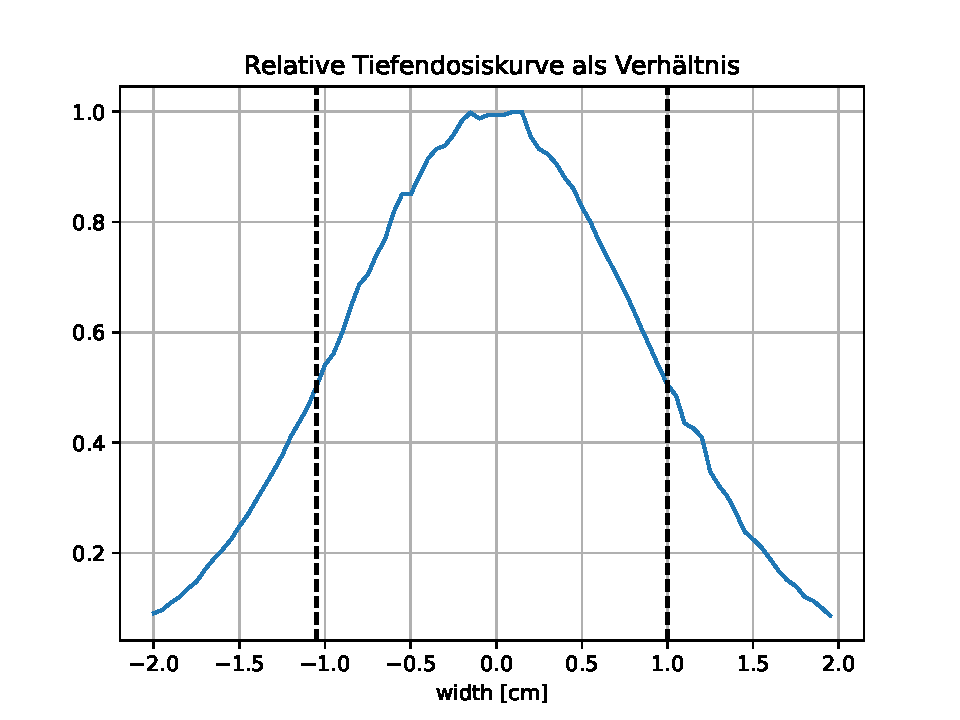
\includegraphics[width = 0.8\textwidth]{../poject/task1/task1a.pdf}
\end{figure}

\subsection{Aufgabe 1 b)}


\section{Aufgabe 2}
\subsection{Aufgabe 2 a)}
Die Grundlegenden Einstellungen, bzw Parameter werden aus der Aufgabe 1 kopiert und können der beiliegenden $.txt$ Datei entnommen wernden.
Um der \enquote{Pencil Beam Scanning Methode} gerecht zu werden, wird der Strahl in 11 Zeitschritten
auf den Mittelpunkt des CTV Zylinders mit je verschiedenen Energien $\left( 140, 145,...,190, 195 \right)$. 
Hierbei wird darauf geachtet, inerhalb des Zylinders zu agieren um die umliegenden OAR nicht unnötiger Strahlung, bei homogener Dosis im CTV, auszusetzen. 
Ein Aufbau von: \newpage Keil \to Streufolie \to Streufolie \to Streufolie \to Kollimator weitet den Strahl auf, wobei die Kollimatoren für laterale 
Sicherheit sorgen. Die Reichweitenmoulierung findet durch die verschiedenen Energien statt.
\begin{figure}
    \centering
    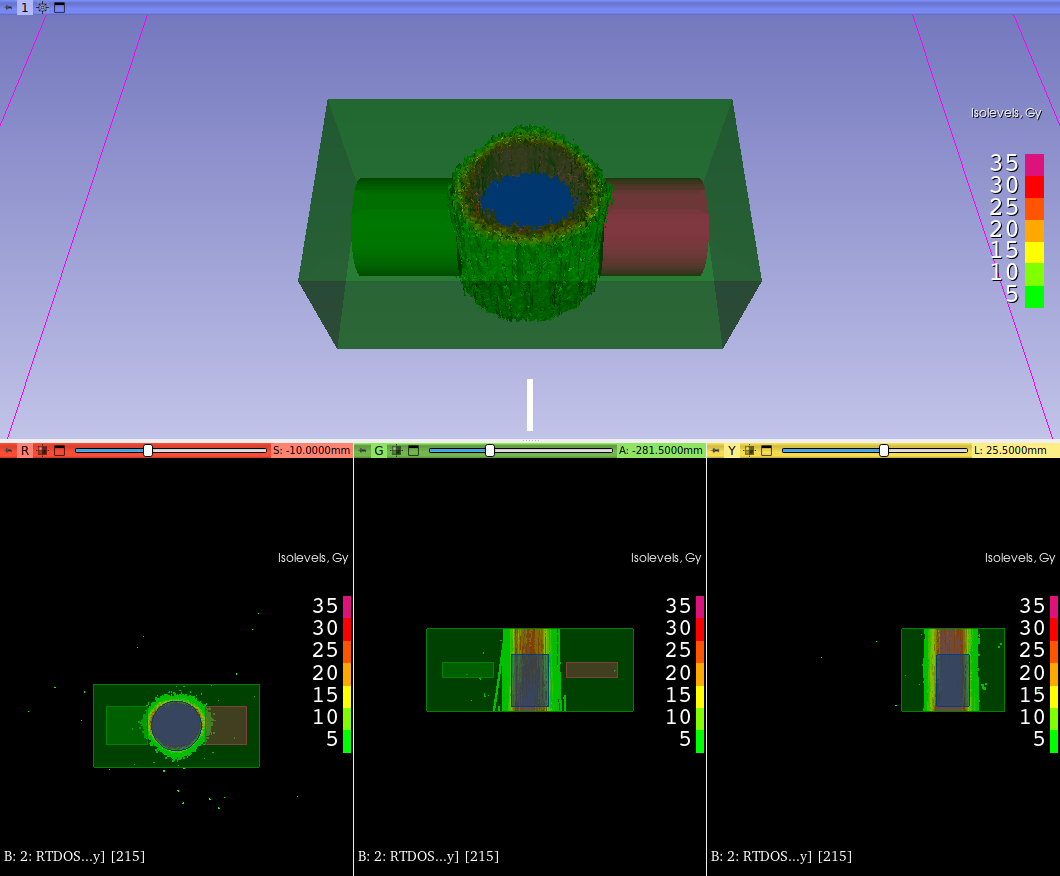
\includegraphics[width= 0.8\textwidth]{content/iso.png}
    \caption{Abgebildet sind die Isodosislinien eines CT Datensatz bei einer Bestrahlung mit einem Protonenstahl in der Pencil Beam Scanning
    Methode.}
    \label{fig:iso}
\end{figure}
Mit dem Simulationswekzeug von \enquote{TOPAS} werden so mehrer Protonen an entsprechender Stelle simuliert wobei die Teilchenanzahl in einer Größenordnung 
von insgesamt $10^8$ liegt. So werden statistische Fehler minimiert. Die deponierte Dosis kann in \enquote{Slicer3D} ausgelesen,
und anschließend durch DICOM manipulation durch den Tag $(3004, 000E)$ auf die gewünschten $60 Gy$ skaliert werden. 
Durch Hinzufügen des Tags (3004, 0002) wird wahlweise noch die Information \enquote{Gy} beigegeben.

\subsection{Aufgabe 2 b)}
Der Abbildung \ref{fig:slicer} ist eine mittlere Dosis von $60 Gy$ zu entnehmen. Die Grafik \ref{fig:dvh} verdeutlich zudem die 
Unterschreitung der Richtlinie von einer maximal Dosis $50 Gy$ und $D_{10\%} < 15 Gy$. 
\begin{figure}
    \centering
    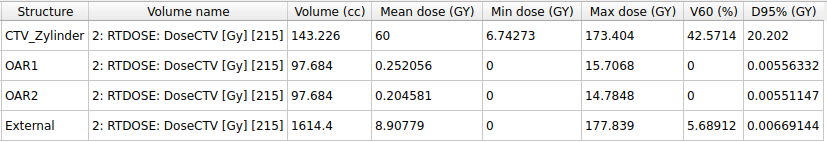
\includegraphics[width  = 0.8\textwidth]{content/slicer.png}
    \caption{Abgebildet sind ausgelesne Dosisinformationen von der Anwendung \enquote{Slicer3D} über die Bestrahlung eines CT Datensatzes.}
    \label{fig:slicer}
\end{figure}
\noindent
Von diesen Richtlinien jedoch abgesehen würde sich die Behandlung bei einem Patienten nicht durchsetzten können. 
Die maximale Dosis, abgelesen in \ref{fig:slicer} würde zu einer direkten Nekrose führen und der Heilungsprozess wäre maßgeblich 
eingeschrkänkt. Zu dem werden lediglich $\approx 42\%$ mit $60Gy$ abgedeckt, was in einem klinischen Standart über $95\%$ liegen sollte.
Alternativ kann in der Planung mit etwaigen Filtern gearbeitet, oder eine Vielfelderplaung etabliert werden
\newpage


%\input{content/Meßwerte.tex}
%\input{content/auswertung.tex}
%\input{content/diskussion.tex}

\newpage
\begin{appendices}
\label{app}
\begin{verbatim}
R80 for TDK1:  7.996688741721854 
 -> resulting in an Energy of : 102.70104559318608
 -> Error Range:  8.00+/-0.08
 -> Error Energy:  102.7+/-0.6
 -> relative Energy:  1.1845374965156918 % 

R80 for TDK2:  10.754966887417218 
 -> resulting in an Energy of : 121.41884571641383
 -> Error Range:  10.75+/-0.11
 -> Error Energy:  121.4+/-0.7
 -> relative Energy:  1.1619391510050547 % 

R80 for TDK3:  14.135761589403973 
 -> resulting in an Energy of : 141.6948195065084
 -> Error Range:  14.14+/-0.14
 -> Error Energy:  141.7+/-0.8
 -> relative Energy:  1.1414771614053059 % 

R80 for TDK4:  17.79801324503311 
 -> resulting in an Energy of : 161.39151682095616
 -> Error Range:  17.80+/-0.18
 -> Error Energy:  161.4+/-0.9
 -> relative Energy:  1.1245113058198264 % 

R80 for TDK5:  21.827814569536425 
 -> resulting in an Energy of : 181.11694407664427
 -> Error Range:  21.83+/-0.21
 -> Error Energy:  181.1+/-1.0
 -> relative Energy:  1.1096916259245062 % 

R80 for TDK6:  26.192052980132452 
 -> resulting in an Energy of : 200.76215169734326
 -> Error Range:  26.19+/-0.25
 -> Error Energy:  200.8+/-1.1
 -> relative Energy:  1.09662200235949 % 

R80 for TDK7:  30.774834437086092 
 -> resulting in an Energy of : 219.9098376025187
 -> Error Range:  30.77+/-0.30
 -> Error Energy:  219.9+/-1.2
 -> relative Energy:  1.0851886759623235 % 
\end{verbatim}
\end{appendices}
\printbibliography{}

\end{document}
